\documentclass[conference]{IEEEtran}
\IEEEoverridecommandlockouts

\usepackage{cite}
\usepackage{amsmath,amssymb,amsfonts}
\usepackage{graphicx}
\usepackage{booktabs}
\usepackage{textcomp}
\usepackage{xcolor}
\usepackage{balance} % equilibra las columnas de la ultima pagina (referencias)
\usepackage[hidelinks]{hyperref}

\graphicspath{{figuras/}}

\begin{document}

% Convención IEEE: trunca las listas de autores con "et al." pasados 6 nombres.
% Debe ir antes de la primera cita para que IEEEtran.bst lo aplique a todas.
\bstctlcite{IEEEexample:BSTcontrol}

\title{Short-Term Photovoltaic Forecasting under Data Scarcity using Leave-One-Plant-Out Evaluation}

\author{\IEEEauthorblockN{C\'esar David Aular Mu\~noz\IEEEauthorrefmark{1}, Sergio Hernández}
\IEEEauthorblockA{Departamento de Computación e Industrias\\
Facultad de Ciencias de la Ingeniería\\
Universidad Cat\'olica del Maule\\
\IEEEauthorrefmark{1} Email: cesaraular02@gmail.com}}

\maketitle

\begin{abstract}
Newly commissioned photovoltaic (PV) plants lack the local generation history that
conventional forecasting models require. The \emph{Cold-Start} generation problem translates into
operational and financial risk for grid operators and small distributed generators. We
investigate whether a single \emph{Cross-Site} deep-learning model, pretrained on many
consolidated plants, can forecast a brand-new plant it has never observed, and how it
compares against strictly local baselines. We benchmark eight configurations such as global
Temporal Fusion Transformer (TFT), Informer, N-HiTS, LSTM and a global XGBoost against
strictly local XGBoost, LSTM and N-HiTS. Evaluation is performed under a Leave-One-Plant-Out (LOPO) protocol that
hides the target PV plant during training and performs inference only using the training plants. The testing protocol
spans 24-hour and autoregressive 7-day horizons over 94 Chilean plants (2014--2024), with
point (RMSE, sMAPE, rRMSE) and probabilistic (90\,\% interval coverage, pinball loss)
metrics, stratified by season. Because the comparison is strictly paired on a shared hourly
grid, we assess it with a Friedman omnibus test followed by pairwise Wilcoxon signed-rank
tests with Holm correction, and we report errors normalised by installed capacity (NRMSE)
alongside rRMSE. Local XGBoost is the most accurate configuration (13.2\,\% median NRMSE,
weekly roll-out) and beats the best global model (global XGBoost, 17.1\,\%) by a significant
margin ($p<10^{-7}$, winning on 77 of 94 plants). No global configuration significantly
outperforms its local counterpart at matched architecture: local N-HiTS beats global N-HiTS
($p<10^{-10}$) and the LSTM pair is statistically indistinguishable ($p=1.00$, 49/45 plants).
The rejection of the global-superiority hypothesis is therefore unambiguous. The value of the
Cross-Site approach lies instead in availability: it is the only paradigm that yields
coherent, calibrated forecasts from the first connected hour, where no local model can exist.
\end{abstract}

\begin{IEEEkeywords}
photovoltaic forecasting, transfer learning, cold-start, deep learning, Temporal Fusion
Transformer, probabilistic forecasting, leave-one-plant-out.
\end{IEEEkeywords}

\section{Introduction}
The accelerated deployment of solar photovoltaic (PV) generation confronts grid operators
with a recurrent operational barrier: a plant that has just been connected to the network
has no operating history from which to learn its production dynamics. Classical PV
forecasting pipelines train a dedicated model per plant on months or years of local
data~\cite{Antonanzas2016}; applied to a freshly commissioned facility they degrade sharply
or cannot be trained at all. This is the \emph{Cold-Start} problem, borrowed from
recommender systems~\cite{Schein2002} where reliable inference is required exactly when
site-specific evidence is absent. The resulting uncertainty inflates balancing costs and
financial exposure for system operators and, acutely, for the small distributed generators
that dominate the recent capacity additions.

A promising solution is to abandon the one-model-per-plant assumption. Instead of learning in
isolation, a single \emph{global} model can be trained across many plants simultaneously,
absorbing shared atmospheric-to-power patterns and transferring them to unseen
sites~\cite{MonteroManso2021,PanYang2010}. Modern attention-based sequence models such as the
Temporal Fusion Transformer (TFT)~\cite{Lim2021}, Informer~\cite{Zhou2021} as well as efficient
hierarchical alternatives such as N-HiTS~\cite{Challu2023} make this \emph{Cross-Site}
strategy technically feasible on multivariate, exogenous-rich PV data. Despite rapid advances
in foundation models for time series~\cite{Ansari2024,Garza2023,Woo2024,Das2024}, a gap
remains in the PV forecasting literature: the performance of global Cross-Site models under a
strictly zero-shot protocol has not been contrasted against strong local baselines evaluated
under an identical protocol.

Much of the literature reports favourable global-transfer results but rarely combines three
demanding conditions at once: (i) a target-plant-blind evaluation with no local fine-tuning,
(ii) a direct contrast against strong local baselines under an identical protocol, and (iii)
a probabilistic characterization of the forecasts. We close this gap. Our contributions are:

\begin{itemize}
\item A reproducible LOPO benchmark of \textbf{eight configurations} (five global, three
strictly local) over \textbf{94 Chilean PV plants}, with formally verified zero-shot
integrity (no feature is a function of the target's own generation).
\item A \textbf{Synthetic Cold-Start} mechanism that initializes the inference
context from a regional efficiency prior computed exclusively on training plants, enabling
inference with zero target history without leakage.
\item A \textbf{point-and-probabilistic} evaluation stratified by season and by evaluation
window, reported with capacity-normalised errors and \textbf{paired statistical tests}
(Friedman + Wilcoxon--Holm) rather than marginal medians alone. It exposes (a) the
statistically significant rejection of the global-superiority hypothesis, (b) the absence of
any architecture at which global transfer significantly beats its local counterpart,
(c) winter as the hardest regime, and (d) a systematic miscalibration of the deep networks'
intervals under transfer.
\end{itemize}

\section{Related Work}
\textbf{PV forecasting.} Deep networks consistently surpass classical statistical methods
for short-term PV power~\cite{Mellit2021,Kumari2021}, and on real solar datasets
attention-based models improve over classical machine learning at the cost of higher data
and compute demand~\cite{Arslan2025}. The TFT has been applied to day-ahead PV forecasting
with quantile outputs and interpretable covariate fusion~\cite{LopezSantos2022}. A recurrent
limitation across these works is the assumption of sufficient local history for training.

\textbf{Global vs.\ local forecasting.} Montero-Manso and Hyndman~\cite{MonteroManso2021}
propose a single global model fitted across related series. The authors show that global model can  generalize at least as
well as many local models, given enough cross-series signal. For intermittent series,
however, the balance between local and global models is not settled~\cite{Damato2026}, and
simple baselines often rival transformers on standard benchmarks~\cite{Zeng2023}.

\textbf{Transfer learning for PV.} Bak et al.~\cite{Bak2025} pretrain on large multi-plant
corpora and fine-tune on the first records of a new site, attenuating error during the first
weeks of operation. Foundation-model approaches push toward pure zero-shot irradiance transfer~\cite{Mishra2025}. Our study
differs by enforcing a strict zero-shot regime \emph{and} comparing against strong local baselines.

\textbf{Zero-shot and few-shot forecasting.} A recent family of pretrained time-series
foundation models targets forecasting on series unseen during training. Chronos tokenises
series and reuses language-model architectures~\cite{Ansari2024}; TimeGPT offers a
zero-shot forecasting API~\cite{Garza2023}; Moirai addresses arbitrary frequencies and
covariates with a masked encoder~\cite{Woo2024}; Lag-Llama builds a decoder-only probabilistic
forecaster over lagged features~\cite{Rasul2023}; and TimesFM shows that a decoder-only model
pretrained on a large corpus is competitive zero-shot~\cite{Das2024}. These models are trained
across heterogeneous domains, whereas our global models are trained within a single domain
(PV) and transferred across \emph{sites}. Few-shot adaptation, in which a handful of local
observations is used to fine-tune, sits between our strict zero-shot setting and the mature
local baselines, and is the natural next step rather than a competing condition here.

\textbf{Uncertainty calibration.} Interval calibration is rarely verified under distribution
shift. Conformal prediction provides distribution-free coverage guarantees under
exchangeability~\cite{Vovk2005}; conformalized quantile regression combines quantile models
with conformal correction~\cite{Romano2019}; EnbPI extends the idea to time series without
exchangeability~\cite{Xu2021}; and adaptive conformal inference retains coverage under
distribution shift by updating the miscoverage level online~\cite{Gibbs2021}. Recalibration of
regression outputs has also been addressed post hoc~\cite{Kuleshov2018}. We do not apply these
methods here; we \emph{measure} whether calibration survives zero-shot transfer, and find that
it does not, which motivates them as future work.

\textbf{Probabilistic forecasting.} Quantile and distributional outputs are standard for
decision-relevant energy forecasting~\cite{Salinas2020,Benidis2022}. We adopt 90\,\%
prediction intervals and evaluate coverage and pinball loss, but crucially examine whether
calibration itself survives the zero-shot transfer.

\section{Methodology}

\subsection{Dataset and Medallion ETL}
The corpus comprises hourly generation from 94 PV plants of the Chilean National Electric
System (2014--2024), dynamic exogenous meteorology (global horizontal irradiance,
temperature, humidity) from the CR2 network, and static geographic attributes (macro-zone,
installed capacity). The plants span the country's steep solar gradient and are grouped into
four macro-zones from the Atacama desert in the north to the south; this grouping is the
static key over which the regional prior is aggregated. A Medallion pipeline
(landing\,$\rightarrow$\,bronze\,$\rightarrow$\,silver\,$\rightarrow$\,gold, Fig.~\ref{fig:medallion})
parses the raw meteorological and generation CSVs, standardizes them to a canonical
$(\mathit{unique\_id},\,\mathit{ds},\,y)$ schema, joins them into a single
\texttt{silver\_unified} table ($\approx$4.37\,M hourly rows), engineers cyclic calendar
features, and imputes \emph{only} exogenous variables (each flagged with an
\texttt{is\_imputed} dummy). Generation $y$ is never imputed: missing hours remain missing,
and metrics score real observations only. A numeric, label-encoded \texttt{silver\_dl} view
feeds the deep networks, while the gold layer materializes one held-out test partition per
plant for the LOPO evaluation. A single orchestrator runs the pipeline behind a pre-run test
gate with idempotent completion markers.

\begin{figure*}[t]
\centering
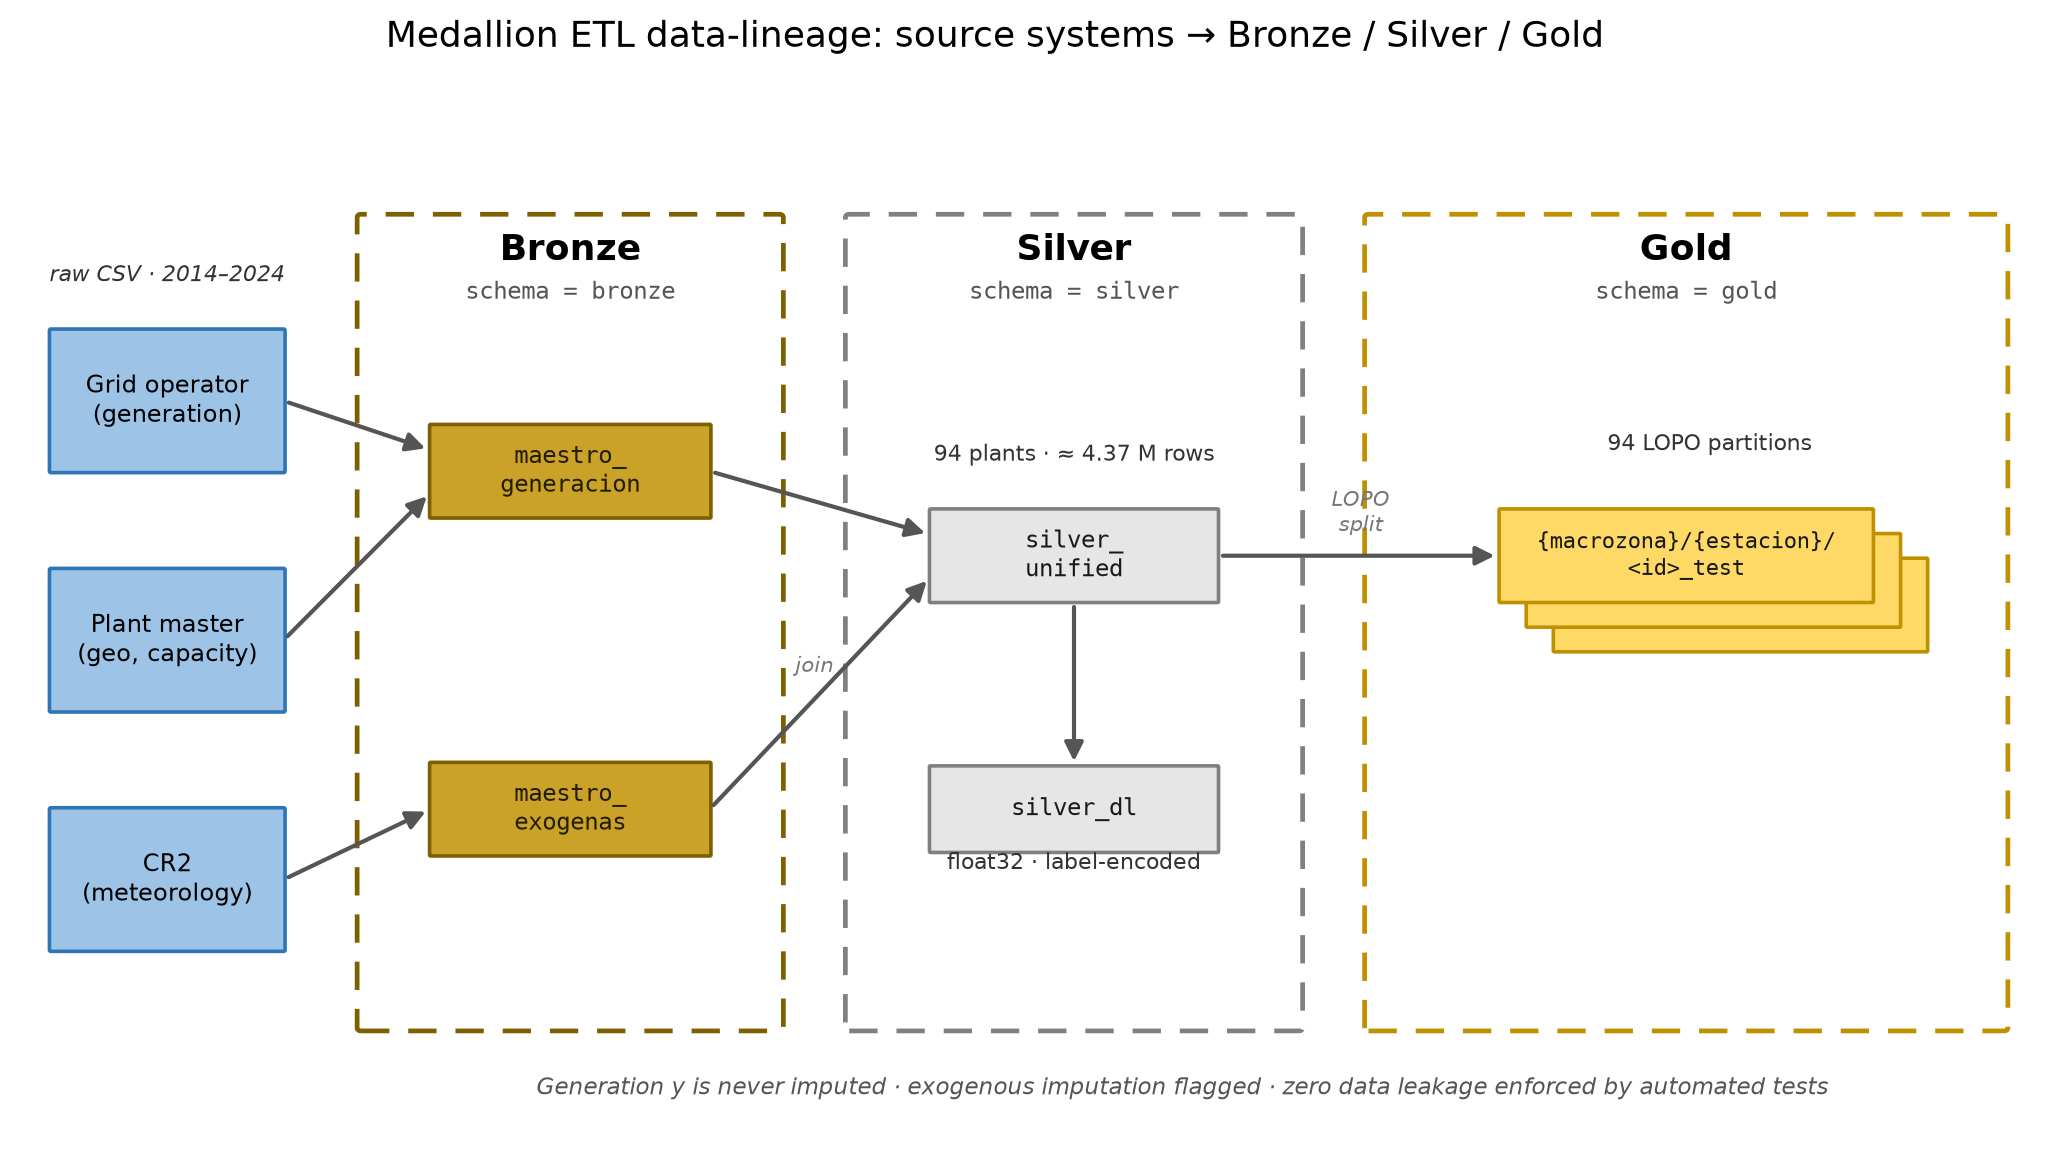
\includegraphics[width=0.9\textwidth]{fig_medallion_en.png}
\caption{Medallion ETL data-lineage. Source systems feed two Bronze master tables, joined
into \texttt{silver\_unified} and its numeric \texttt{silver\_dl} view; the gold layer holds
one LOPO test partition per plant. Generation is never imputed, and zero leakage is enforced
by automated tests.}
\label{fig:medallion}
\end{figure*}

\subsection{LOPO Protocol and Zero-Shot Integrity}
Evaluation follows a Leave-One-Plant-Out design. For each target plant, the global models
are trained on the full 2014--2024 history of the remaining $N{-}1$ plants; the target is
\emph{completely invisible} during training. Zero-shot integrity is a hard constraint: no
predictor may be a function of the target's own $y$. This is enforced by automated tests and
was decisive---an early efficiency prior computed per-row from the target
($\mathrm{corr}=1.0$ with $y$) produced a fake $\sim$0.8\,\% rRMSE that collapsed to the
honest $\sim$56\,\% once removed.

\subsection{Synthetic Cold-Start Context}
Deep models require a context window to initialize inference, which a new plant cannot
provide. We seed it synthetically:
\begin{equation}
\hat{y}_{\text{seed}}(t) = \mathrm{capacity}\cdot PR_{\text{regional}}\cdot s(t),
\end{equation}
where $s(t)$ is a deterministic solar profile and $PR_{\text{regional}}$ is a performance
ratio aggregated by macro-zone and season \emph{over the training plants only}. Only known or
forecastable exogenous weather and static geography use the target's real values; the
generation context is entirely synthetic (Fig.~\ref{fig:method}).

\subsection{Models and Probabilistic Output}
We evaluate five global configurations---TFT~\cite{Lim2021}, Informer~\cite{Zhou2021},
N-HiTS~\cite{Challu2023}, LSTM~\cite{Hochreiter1997} and a global gradient-boosted
XGBoost~\cite{Chen2016}---and three strictly local baselines (XGBoost, LSTM, N-HiTS) trained
only on the target's own history with all evaluation windows excluded. The four deep
architectures span complementary inductive biases: the TFT combines variable-selection
networks with interpretable multi-head attention and gating; the Informer replaces full
attention with a ProbSparse mechanism for long sequences; N-HiTS performs hierarchical
multi-rate interpolation; and the LSTM is a strong recurrent baseline. Deep models are
trained with NeuralForecast in \texttt{fp32} on a 6\,GB GPU under an epoch-based step budget
capped per strategy. Every model emits P5/P50/P95 quantiles (90\,\% intervals), and
predictions are physically constrained ($\hat{y}\!\geq\!0$; forced to zero at night).

\textbf{Data separation and hyperparameter selection.} The holdout in LOPO is \emph{across
plants}, not across time: for a given target, the training set is the complete 2014--2024
history of the other $N{-}1$ plants, and the test set is the target's evaluation window.
Early stopping uses the last 168 hours of each training series as a validation split, so
validation is temporally posterior to the data used for the gradient updates of that series.
Hyperparameters are searched once per architecture (Optuna, on a fixed development subset of
training plants) and reused across all folds. This reuse is a deliberate compute trade-off
and constitutes \emph{parameter-level} information sharing across folds. We bound its effect
rather than assert it away: the search space is small (learning rate, hidden size, number of
layers), the same configuration is applied to every fold so no fold is individually tuned on
its own target, and the ranking we report is driven by differences far larger than the spread
observed across the tuning trials. It remains a limitation, and a per-fold search would be
the strictly correct protocol.

\textbf{Temporal causality of the local baselines.} The local baselines are trained on the
target plant's full history \emph{with all evaluation windows removed}---Raw, Operational and
the four Seasonal windows---rather than on data strictly preceding each window. Lags that
would reach into a removed window are masked, so no evaluation target leaks in as a feature;
but the training set does include hours chronologically \emph{after} the window being
predicted. This is a deliberate choice: the local baseline is meant to represent the mature
model an operator would eventually hold once the plant has accumulated history, which is the
strongest possible opponent for the Cross-Site approach. It is nonetheless an optimistic
setting for the local side. The global side carries a mirror-image advantage: LOPO hides the
target plant but not the calendar, so a global model does observe the same hours at
neighbouring plants of the same macro-zone. Both biases favour the conclusion being tested
against---the local side is flattered and it wins, while the global side is flattered and it
still loses---so they reinforce rather than undermine the rejection reported in
Section~\ref{sec:stats}. A strictly causal rolling-origin protocol is left as future work.

\subsection{Evaluation Windows and Metrics}
\label{sec:windows}
Two horizons are scored: \emph{day1} (24\,h direct) and \emph{rollout7d} (7 autoregressive
days feeding back the predicted median). Because early series often contain a
\emph{commissioning ramp} of null generation, we report a window sensitivity analysis
(Fig.~\ref{fig:method}): \emph{Raw} (from the first recorded hour, ramp included),
\emph{Operational} (from first sustained production) and four \emph{Seasonal} windows
starting in each season, drawn from the plant's own later history. Point metrics are RMSE,
sMAPE and two normalisations of the RMSE. The first, rRMSE, divides by the window's mean
hourly generation; because that mean includes null night hours it inflates the index, and
values above 100\,\% are expected rather than anomalous. We retain rRMSE for continuity with
the thesis this work condenses, but we add
\begin{equation}
\mathrm{NRMSE} = \frac{\mathrm{RMSE}}{P_{\mathrm{inst}}}\times 100,
\end{equation}
normalised by the plant's installed capacity $P_{\mathrm{inst}}$, which is bounded, directly
interpretable as a percentage of nameplate power, and comparable across plants of very
different size (0.3--200\,MW here). NRMSE is also the metric on which the statistical tests
are run, because it is defined for every plant, whereas rRMSE is undefined when a window's
mean generation is zero. Probabilistic quality uses 90\,\% coverage and pinball loss; we
report \emph{diurnal} coverage (hours with $y>0$) as the honest measure, since the physical
night-zero forcing yields trivial nocturnal hits. Reported cells are medians over plants,
with interquartile ranges given for the headline metric.

\textbf{What the global--local comparison is for.} The two families are not evaluated under
equivalent information: a global model sees no data at all from the target plant, whereas a
local baseline sees that plant's own history. The comparison is therefore not a like-for-like
contest but a deliberate test of a practical question---\emph{does knowledge transferred from
other plants substitute for the plant's own history?} We report it at two levels: against the
strongest available local baseline, which bounds what the operator gives up by using transfer,
and at \emph{matched architecture} (global vs.\ local LSTM, global vs.\ local N-HiTS), which
isolates the effect of the training regime from that of the model family.

\begin{figure}[t]
\centering
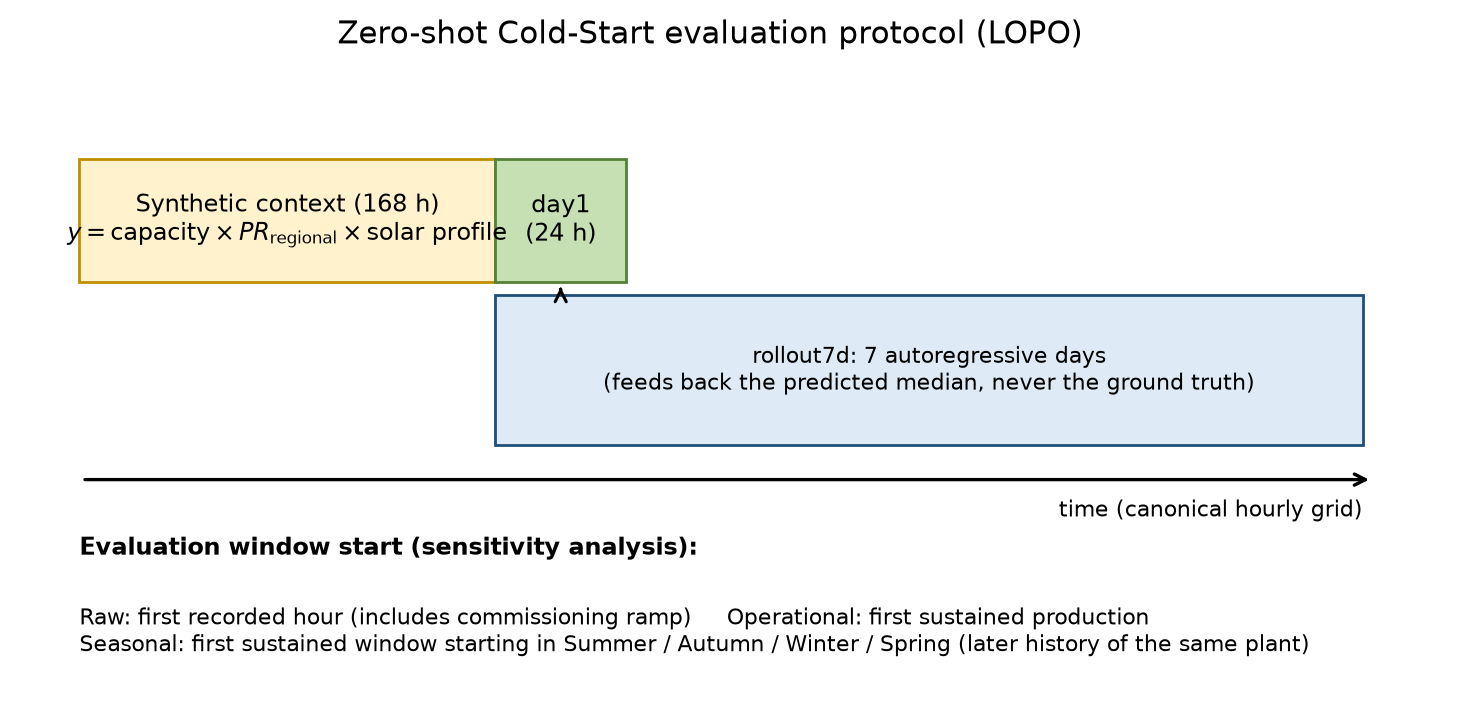
\includegraphics[width=\columnwidth]{fig_method_en.png}
\caption{Zero-shot Cold-Start evaluation protocol. A 168-hour synthetic context seeds the
inference; the model then predicts the \emph{day1} (24\,h) and \emph{rollout7d} horizons.
The window start defines the Raw/Operational/Seasonal sensitivity analysis.}
\label{fig:method}
\end{figure}

\section{Results}
Results correspond to the \emph{total}-scale run: LOPO over the 94 target plants, global
models trained on the complete $N{-}1$ history. Table~\ref{tab:main} reports the cold-start
window for all 94 plants; Fig.~\ref{fig:results} visualizes the weekly roll-out ranking.

\begin{table*}[t]
\centering
\caption{Median performance by configuration over all \textbf{94 plants}, cold-start window,
sorted by NRMSE. For the 33 plants with a commissioning ramp longer than 24\,h the
Operational window is used; for the remaining 61, whose sustained production starts within
24\,h of the first record, the Raw window already begins in sustained production and is used
instead. rRMSE normalises by the window's mean generation, NRMSE by installed capacity;
IQR is the interquartile range of the roll-out NRMSE across plants. Cov$_{90}$ is diurnal
coverage of the 90\,\% interval and pinball P95 is in MWh. Best value per column in
\textbf{bold}.}
\label{tab:main}
\begin{tabular}{llccccccc}
\toprule
 &  & \multicolumn{2}{c}{rRMSE (\%)} & \multicolumn{2}{c}{NRMSE (\% cap.)} & & & \\
\cmidrule(lr){3-4}\cmidrule(lr){5-6}
Model & Scope & day1 & roll7d & day1 & roll7d & IQR$_{\text{NRMSE}}$ & Cov$_{90}$ & Pinball \\
\midrule
XGBoost & Local & \textbf{45.6} & \textbf{59.9} & \textbf{9.5} & \textbf{13.2} & [8.7, 17.9] & 0.86 & \textbf{0.035} \\
XGBoost & Global & 64.0 & 75.1 & 15.6 & 17.1 & [13.6, 21.6] & 0.97 & 0.092 \\
N-HiTS & Local & 62.3 & 85.2 & 14.2 & 17.6 & [13.4, 22.7] & 0.72 & 0.096 \\
Informer & Global & 96.6 & 106.5 & 21.0 & 22.8 & [19.3, 31.6] & 0.64 & 0.115 \\
TFT & Global & 105.1 & 112.7 & 22.0 & 23.6 & [18.9, 29.0] & 0.38 & 0.158 \\
LSTM & Local & 102.6 & 128.8 & 16.3 & 23.9 & [16.1, 33.8] & 0.72 & 0.235 \\
LSTM & Global & 99.7 & 108.6 & 22.6 & 24.8 & [20.9, 31.8] & 0.53 & 0.159 \\
N-HiTS & Global & 129.8 & 148.2 & 28.6 & 30.7 & [21.6, 42.6] & 0.37 & 0.372 \\
\bottomrule
\end{tabular}
\end{table*}

\subsection{Point Accuracy}
Three readings emerge from the weekly roll-out. First, \textbf{local XGBoost} is the most
accurate configuration (13.2\,\% median NRMSE, i.e.\ an RMSE of 13\,\% of nameplate power),
followed by \textbf{global XGBoost} (17.1\,\%), the best Cross-Site model. Second, the deep
networks form a clearly worse group (22.8--30.7\,\% NRMSE) in which \textbf{N-HiTS global} is
the weakest; the ordering is consistent with the caution that attention can be
over-provisioned relative to simpler baselines~\cite{Zeng2023}. Third, the degradation from
\emph{day1} to the weekly roll-out is moderate across all families, indicating that
autoregressive median feedback does not destabilize the forecasts.

The two normalisations also illustrate why the choice matters. Ranked by rRMSE, global LSTM
(108.6\,\%) appears clearly ahead of local LSTM (128.8\,\%); ranked by NRMSE the order
reverses (24.8\,\% vs.\ 23.9\,\%). Marginal medians of a ratio whose denominator varies by
plant are not a safe basis for ranking, which is precisely why we turn to paired tests.

\begin{figure}[t]
\centering
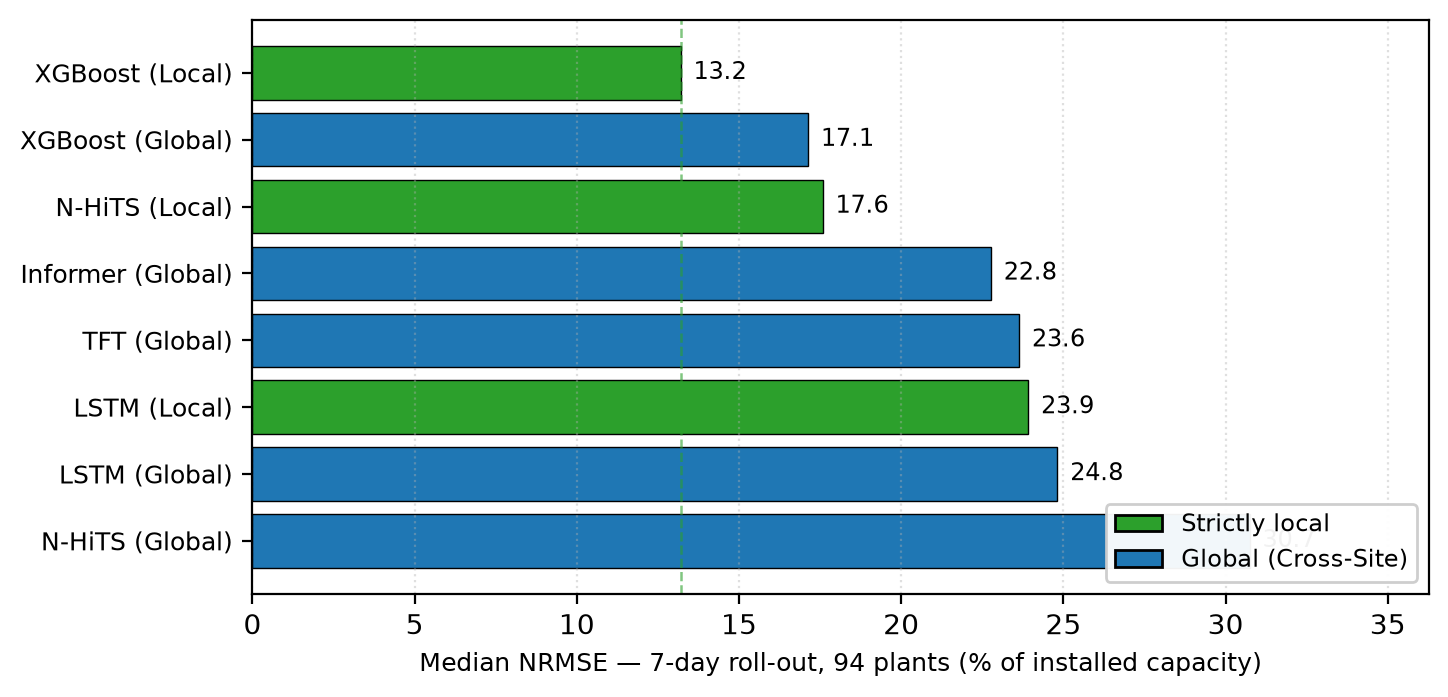
\includegraphics[width=\columnwidth]{fig_results_en.png}
\caption{Median NRMSE (7-day roll-out, cold-start window, 94 plants) per configuration, as a
percentage of installed capacity. Local models in green, global Cross-Site models in blue;
the dashed line marks the best local baseline.}
\label{fig:results}
\end{figure}

\subsection{Commissioning-Ramp Window Sensitivity}
Only 33 of the 94 plants exhibit a commissioning ramp longer than 24\,h; for the rest the
Raw and Operational windows coincide. On the aggregate median the two definitions differ only
moderately, but on plants with a ramp the Raw window is distorted: starting the evaluation
over weeks of null generation drives the window mean toward zero and makes rRMSE undefined.
Reporting both definitions is therefore deliberate---Raw is faithful to the historical record,
whereas Operational yields interpretable metrics for a plant already in commercial operation
and is the window used for the headline comparison.

\subsection{Seasonal Sensitivity}
For every plant we build Cold-Start windows starting in each of the four seasons, taken from
its own post-commissioning history (independent of the actual connection season). Winter is
\textbf{systematically the hardest season for every architecture} (Table~\ref{tab:seasonal}):
in the weekly roll-out, global XGBoost rises from 51.8\,\% (summer) to 133.5\,\% (winter) and
local XGBoost from 40.5\,\% to 114.8\,\%. Greater cloud variability and lower mean winter
irradiance weaken the deterministic solar signal and amplify the relative weight of errors,
with a direct operational implication: the forecast uncertainty of a newly connected plant
depends strongly on the season of its commissioning.

\begin{table}[t]
\centering
\caption{Median rRMSE (\%) of the 7-day roll-out by season in which the evaluation window
starts, for all eight configurations.}
\label{tab:seasonal}
\begin{tabular}{llcccc}
\toprule
Model & Scope & Summer & Autumn & Winter & Spring \\
\midrule
XGBoost & Local & 40.5 & 35.9 & 114.8 & 101.5 \\
XGBoost & Global & 51.8 & 53.7 & 133.5 & 106.1 \\
N-HiTS & Local & 66.0 & 74.0 & 143.5 & 118.1 \\
N-HiTS & Global & 114.0 & 130.3 & 188.7 & 148.9 \\
LSTM & Local & 94.1 & 139.6 & 166.1 & 155.1 \\
LSTM & Global & 93.9 & 97.0 & 186.3 & 136.2 \\
TFT & Global & 87.7 & 102.0 & 168.8 & 130.9 \\
Informer & Global & 87.9 & 92.9 & 172.0 & 137.0 \\
\midrule
\textit{plants} & & 94 & 92 & 93 & 94 \\
\bottomrule
\end{tabular}
\end{table}

\begin{figure*}[t]
\centering
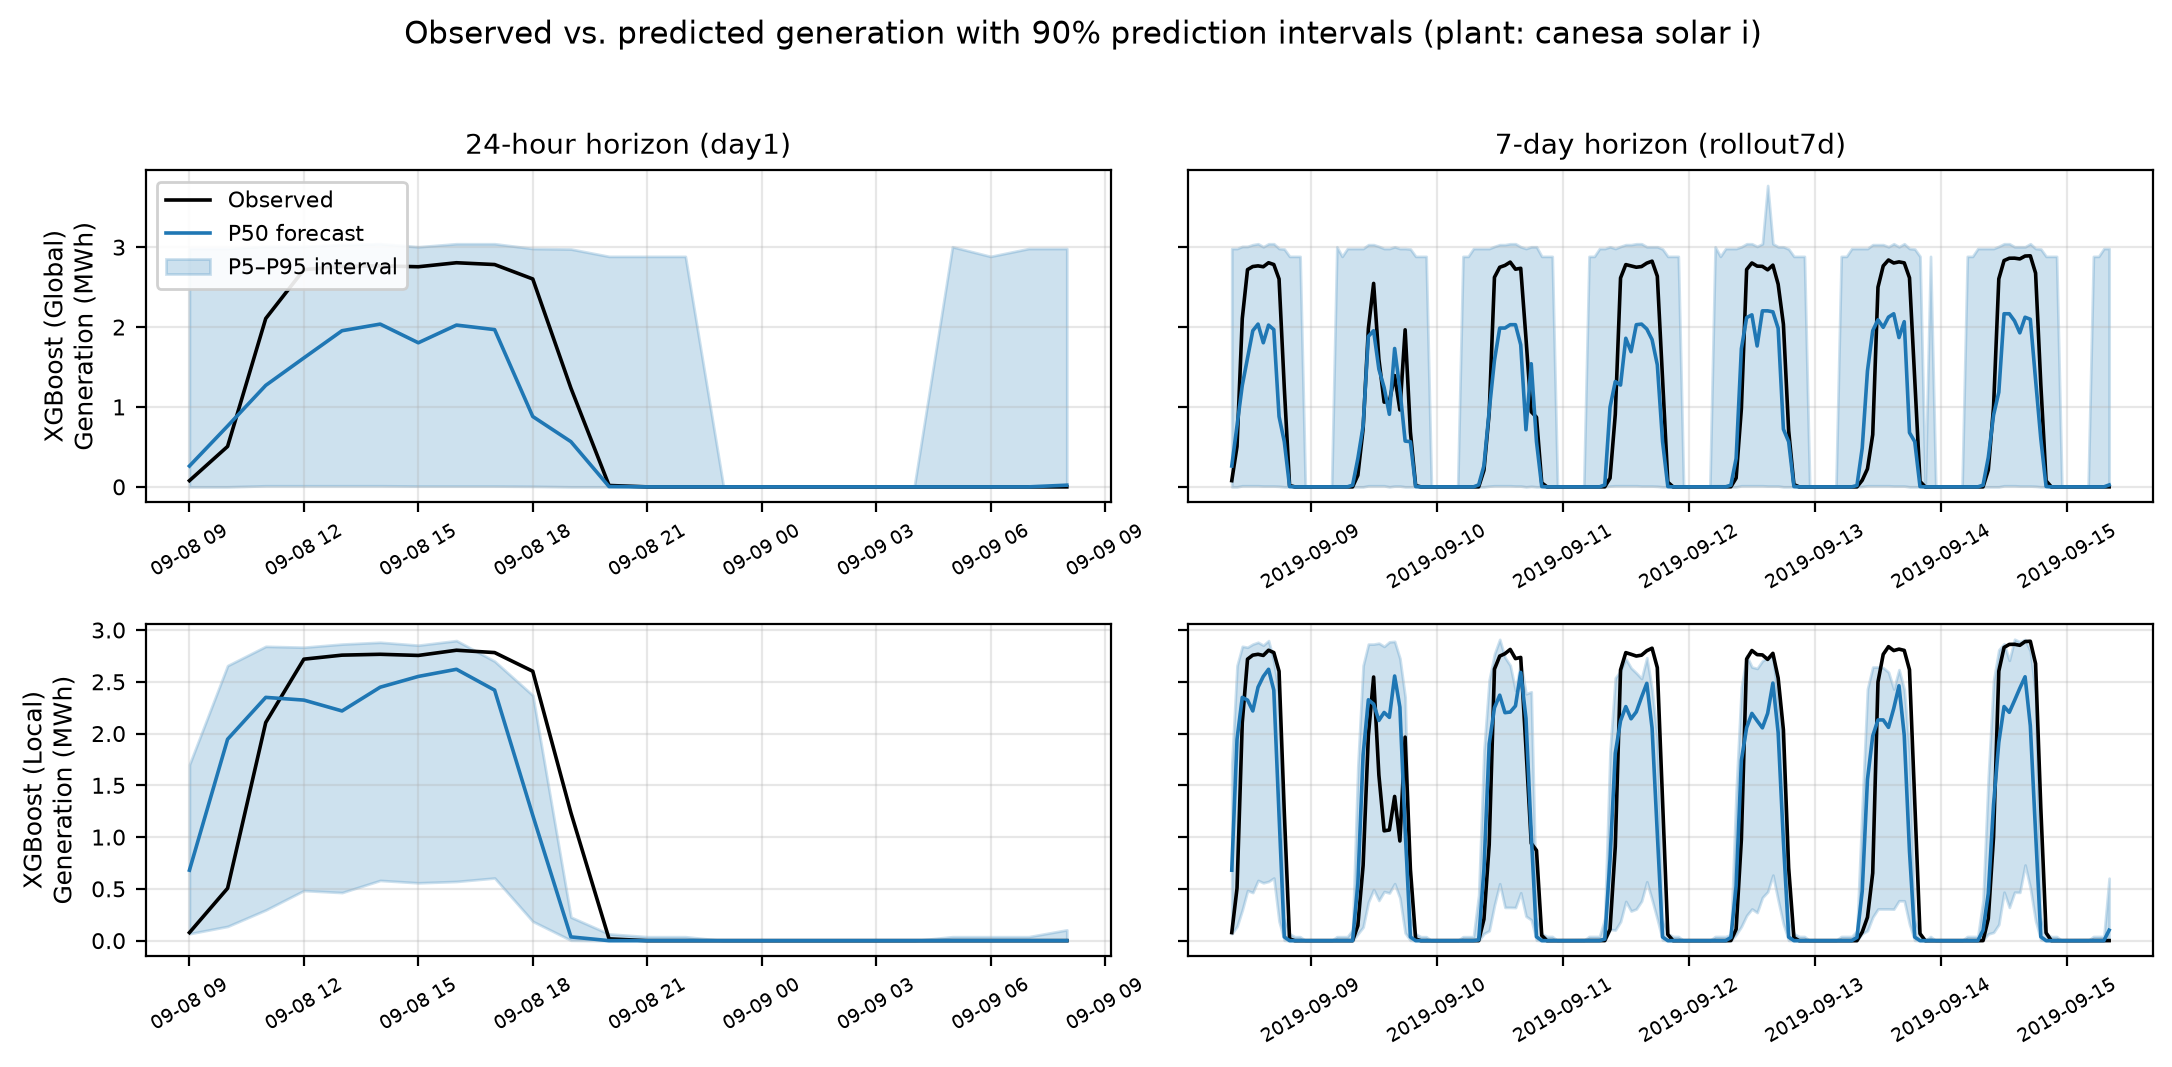
\includegraphics[width=0.92\textwidth]{fig_timeseries_en.png}
\caption{Observed vs.\ predicted generation with 90\,\% prediction intervals for the same
plant and window, at the 24-hour (left) and 7-day (right) horizons. Top: global XGBoost,
whose median under-forecasts the peaks and whose bands are far too wide (over-coverage).
Bottom: local XGBoost, which tracks the daily cycle closely with near-nominal bands.}
\label{fig:timeseries}
\end{figure*}

\subsection{Probabilistic Calibration}
No paradigm calibrates its intervals ideally under the Cold-Start protocol, with deviations
in opposite directions from the 90\,\% nominal (Table~\ref{tab:main}, Cov$_{90}$). Evaluated
on productive hours, the global deep networks are clearly \textbf{under-calibrated} (global
LSTM 0.53, Informer 0.64, TFT 0.38, N-HiTS 0.37): their bands are too narrow. Global XGBoost,
at the opposite extreme, \textbf{over-covers} (0.97)---bands so wide they rarely fail but lose
operational value, a defect symmetric to the networks', not a virtue. The closest to nominal
is \textbf{local XGBoost} (0.86), whose superiority is confirmed by a much smaller pinball
P95 (0.035 vs.\ 0.092\,MWh for global). The networks' behaviour follows from the design:
each series' local scaler is fit on the synthetic context, whose variance (an idealized
solar profile) is below the real plant variability, producing narrow bands; the local deep
baselines, which see real context, improve (LSTM local and N-HiTS local both 0.72).
Post-hoc recalibration---conformalized quantile regression~\cite{Romano2019}, time-series
conformal intervals~\cite{Xu2021} or adaptive conformal inference under
shift~\cite{Gibbs2021}---is a clear line of future work.

\subsection{Statistical Significance}
\label{sec:stats}
Because every configuration is evaluated on the same plants over the same canonical hourly
grid, the design is fully paired and balanced ($94$ plants $\times$ $8$ configurations), which
is the setting in which rank-based comparisons over multiple datasets
apply~\cite{Demsar2006}. We run a Friedman omnibus test on the roll-out NRMSE followed by all
$28$ pairwise Wilcoxon signed-rank tests with Holm correction.

The omnibus test rejects the null of equal performance decisively
($\chi^2=260.7$, $p<10^{-50}$). Mean ranks (1 = best) order the configurations as local
XGBoost $1.80$, local N-HiTS $3.32$, global XGBoost $3.34$, TFT $5.10$, Informer $5.15$,
local LSTM $5.30$, global LSTM $5.41$, global N-HiTS $6.59$. Counting per-plant winners gives
the same picture: local XGBoost is best on $60$ of $94$ plants, global XGBoost on $15$, local
N-HiTS on $10$, and the remaining four configurations on $9$ plants combined.

Table~\ref{tab:stats} reports the contrasts that bear on the hypothesis. Local XGBoost beats
global XGBoost on $77$ of $94$ plants ($p<10^{-7}$), so the headline rejection is significant
and not an artifact of aggregation. At matched architecture the picture is now unambiguous:
local N-HiTS beats global N-HiTS on $88$ of $94$ plants ($p<10^{-10}$), and the LSTM pair is
\textbf{statistically indistinguishable} (median paired difference $0.3$ NRMSE points,
$49$/$45$ plants, $p=1.00$ after correction). \emph{There is no architecture at which global
transfer significantly outperforms its local counterpart.}

\begin{table}[t]
\centering
\caption{Key contrasts on roll-out NRMSE over 94 plants. Paired Wilcoxon signed-rank with
Holm correction; ``Wins'' counts plants on which the first configuration is better. A dash
means the difference is not significant at $\alpha=0.05$.}
\label{tab:stats}
\footnotesize
\begin{tabular}{llrrr}
\toprule
Contrast & Better & $\Delta$ & Wins & $p$ \\
\midrule
XGB: local vs.\ global & local & 3.7 & 77/17 & $<10^{-4}$ \\
LSTM: global vs.\ local & --- & 0.3 & 49/45 & $1.000$ \\
N-HiTS: global vs.\ local & local & 13.8 & 6/88 & $<10^{-4}$ \\
Global: XGB vs.\ LSTM & XGB global & 9.0 & 75/19 & $<10^{-4}$ \\
\bottomrule
\end{tabular}
\end{table}

This result corrects a reading that marginal medians invite. On the earlier operational
subset, global LSTM showed a much better median rRMSE than local LSTM ($118.2$ vs.\
$146.9$\,\%), which suggested a genuine advantage for transfer at matched architecture. The
paired difference tells a different story: the median of the per-plant differences is
essentially zero and slightly favours the local model. The gap between the two medians was
driven by a minority of plants on which the local LSTM fails badly, not by a systematic
advantage of the global one. The hypothesis is therefore rejected without the nuance we
previously claimed.

The operational value of the global model is consequently not accuracy but
\emph{availability}: the local paradigm needs months of accumulated data, whereas the global
model forecasts usably from the first connected hour, a regime in which no local competitor
exists.

Fig.~\ref{fig:timeseries} makes the same contrast visible at the series level for a
representative plant: the global model reproduces the diurnal shape from weather and static
geography alone, but systematically under-shoots the peaks and hedges with very wide
intervals, whereas the local model tracks both the level and the shape with much tighter
bands.

\section{Discussion}
The results show that Cross-Site transfer retains value in a pure cold start scenario. Several factors may affect the
global models' performance and define the roadmap. The global model
ran strictly zero-shot while the local baselines that beat it observe real site data; a
two-stage pretrain-then-finetune scheme should close much of the gap as history accrues.
Also, the models treat PV as a continuous signal, whereas
it is intrinsically intermittent (deterministic night zeros, stochastic cloud gaps);
explicit intermittency masks in the attention mechanism could redirect representational
capacity to the productive signal. \emph{Corpus scale and compute:} 94 plants and a 6\,GB
training budget may under-serve the higher-capacity TFT/Informer, offering an alternative
explanation for their being outperformed by simpler models. Finally, \emph{Interval recalibration}
under transfer (conformal methods) is needed before operational deployment.

Beyond the benchmark, four takeaways can be generalized
to any cold-start forecasting study. (1) Commissioning ramps of null generation distort
relative metrics unless the window is defined from sustained production, which motivated our
Raw/Operational split. (2) Winter is systematically the hardest regime, doubling or tripling
summer errors across all architectures. (3) Probabilistic calibration does not transfer to
the deep networks under a synthetic context, whereas quantile gradient boosting calibrates
well---a critical distinction for electricity-market use. (4) Target integrity requires never
imputing missing generation and is essential to metric honesty, in contrast to the common
practice of zero-filling.

\textbf{Limitations.} The study is zero-shot by design, with no fine-tuning arm, so it bounds
what transfer achieves without any local adaptation rather than what a few-shot scheme could
reach. The local baselines are trained non-causally with respect to their evaluation window
(Section~\ref{sec:windows}), which favours them; a rolling-origin protocol would settle the
margin exactly. Hyperparameters are shared across folds. The rRMSE normalisation inflates
absolute magnitudes and is meaningful only in relative comparison, which is why NRMSE and the
paired tests carry the conclusions. Operational MLOps deployment is out of scope.

\section{Conclusion}
We benchmarked global Cross-Site transfer against strictly local baselines for cold-start PV
forecasting under a target-blind LOPO protocol over 94 Chilean plants, and assessed the
comparison with paired statistical tests rather than marginal medians alone. The
global-superiority hypothesis is rejected, and the rejection is statistically significant: a
local XGBoost beats the best global configuration on 77 of 94 plants ($p<10^{-7}$), and no
architecture shows a significant advantage for global transfer over its local counterpart.
The value of the Cross-Site paradigm is therefore not accuracy but availability: in the pure
cold-start regime it is the only approach that produces coherent, immediately usable
forecasts, because no local model can be trained at all. Winter is the hardest season, and
the deep networks' probabilistic intervals require recalibration under transfer. The
contribution is not to crown an absolute winner but to quantify rigorously the trade-off
between \emph{immediate availability} and \emph{asymptotic accuracy} that governs paradigm
choice during the commissioning of a new solar plant.

\section*{Reproducibility}
The medallion ETL, the LOPO split and all eight configurations are driven by a single
orchestrator behind an automated test gate that halts the run on any failure; every metric is
computed only over real observations on a shared canonical hourly grid, so the eight models
are compared in a strictly paired fashion. Idempotent completion markers make long runs
resumable, and the regional prior is recomputed inside each fold to preserve zero-shot
integrity. The source code, the per-plant metric tables underlying every figure and table in
this paper, and the scripts that compute the statistical tests are available from the authors
upon request.

\section*{Acknowledgment}
This paper condenses the first author's undergraduate thesis at Universidad Cat\'olica del
Maule, supervised by the second author. AI-assisted tools supported drafting and figure
preparation; all content, data and results were produced and verified by the authors.


\balance
\bibliographystyle{IEEEtran}
\bibliography{paper}

\end{document}
